\documentclass[t]{beamer}
\usetheme{Copenhagen}
\setbeamertemplate{headline}{} % remove toc from headers
\beamertemplatenavigationsymbolsempty

\usepackage{amsmath, array, tikz, bm, pgfplots, tcolorbox, graphicx, venndiagram, color, colortbl}
\pgfplotsset{compat = 1.16}
\usepgfplotslibrary{statistics}
\usetikzlibrary{calc}

\title{Histograms}
\author{}
\date{}

\AtBeginSection[]
{
  \begin{frame}
    \frametitle{Objectives}
    \tableofcontents[currentsection]
  \end{frame}
}

\begin{document}

\begin{frame} 
\maketitle
\end{frame}

\section{Create a frequency distribution for quantitative data}

\begin{frame}{Frequency Distribution for Quantitative Data}
The weights (in pounds) of 25 husky dogs are shown below:
\begin{center}
\begin{tabular}{ccccc}
53 & 46 & 44 & 47 & 50 \\
49 & 47 & 44 & 61 & 44 \\
35 & 46 & 49 & 51 & 48 \\
50 & 52 & 44 & 50 & 47 \\
58 & 47 & 52 & 37 & 54 \\
\end{tabular}
\end{center}
Suppose we want to create a frequency distribution for the weights of these awesome dogs. \newline\\	\pause

Since this data is quantitative, we are going to have to decide what each of our ranges of weights in our classes is going to be. 
\end{frame}

\begin{frame}{Definitions for Quantitative Data}
The smallest value (weight in our case) in each class (table row) is called the {\color{blue}\textbf{lower class limit}}. \newline\\	\pause

The largest value in each class is the {\color{blue}\textbf{upper class limit}}. \newline\\ \pause 

Typically, the closer the lower and upper class limits are in value, the more classes we will need. \newline\\	\pause

The difference between two consecutive lower class limits is called the {\color{blue}\textbf{class width}}.	\newline\\	\pause

Let's create a frequency distribution for the dog weights using a class width of 5 pounds.
\end{frame}

\begin{frame}{Frequency Distribution of the Weights of Adorable Huskies}
\begin{center}
\begin{tabular}{c|c}
\textbf{Weight} & \textbf{Frequency} \\ \hline
35 -- 39 & 2 \\
40 -- 44 & 4 \\
45 -- 49 & 9 \\
50 -- 54 & 8 \\
55 -- 59 & 1 \\
60 -- 64 & 1 \\
\end{tabular}
\end{center}
\pause
In the above table, we are only considering integer weight values.	\newline\\	\pause

However, any dog that weighs at or above 39.5 pounds, but less than 44.5 pounds, would have to go into the 40 -- 44 pound class. \newline\\	\pause

Going a half of another decimal place below the lower class limit and above the upper class limits give us the {\color{blue}\textbf{class boundaries}}.
\end{frame}

\section{Create and interpret histograms}

\begin{frame}{Histograms of Quantitative Data}
We can use class limits to create a histogram of the data.	\newline\\	\pause

A histogram is like a bar graph in which there are no gaps between classes.		\pause

\begin{center}
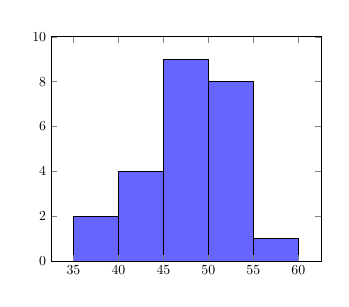
\begin{tikzpicture}[scale=0.5]
\begin{axis}[
ymin = 0, ymax = 10, area style
]
\addplot[ybar interval, fill=blue!60, mark=no] plot coordinates {(35,2) (40,4) (45,9) (50,8) (55,1) (60,1)};
\end{axis}
\end{tikzpicture}
\end{center}
\pause We can also use class midpoints when graphing histograms. \pause \newline\\

To find the class midpoint, add the lower class limit and upper class limit. Then divide by two.
\end{frame}

\begin{frame}{Relative Frequency Histogram}
We can even make a relative frequency histogram of a data set.	\newline\\	\pause

The total area of all rectangles will equal 100\%.	\newline\\	\pause
\begin{center}
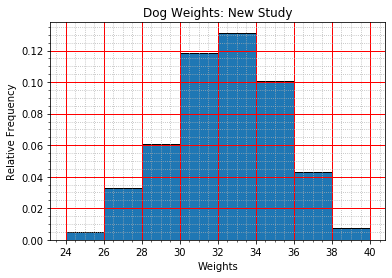
\includegraphics[scale=0.55]{../Images/dog_weights_relfreq_hist.png}
\end{center}
\end{frame}

\begin{frame}{Example 1}
Answer each given the histogram below.
\begin{center}
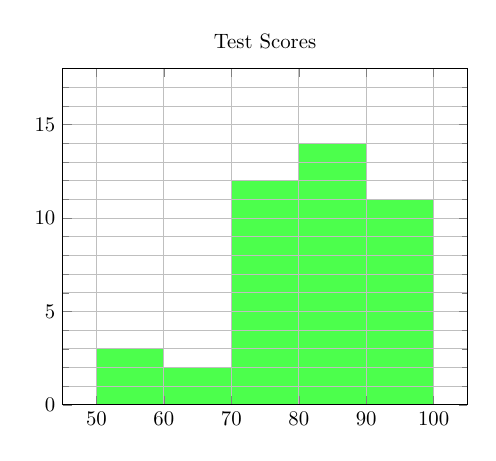
\begin{tikzpicture}[scale=0.75]
\begin{axis}[
    ymin=0, ymax=18,
    minor y tick num = 4,
    area style, grid=both, title=Test Scores
    ]
\addplot+[ybar interval,mark=no,fill=green!70] plot coordinates { (50, 3) (60, 2) (70, 12) (80, 14) (90, 11) (100, 9)};
\end{axis}
\end{tikzpicture}
\end{center}
(a) What is the class width?	\quad \onslide<2->{10}
\end{frame}

\begin{frame}{Example 1}
(b) What is the class midpoint of the 4th class?	\quad \onslide<2->{85}
\begin{center}
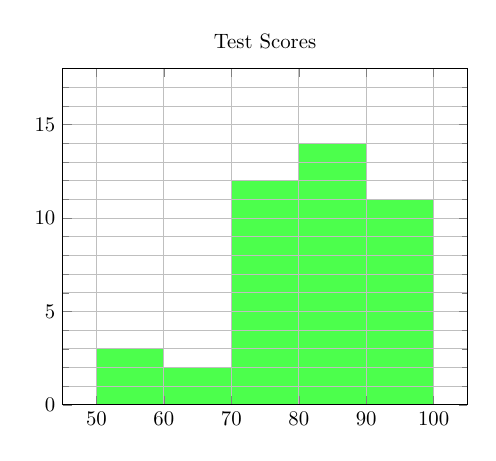
\begin{tikzpicture}[scale=0.75]
\begin{axis}[
    ymin=0, ymax=18,
    minor y tick num = 4,
    area style, grid=both, title=Test Scores
    ]
\addplot+[ybar interval,mark=no,fill=green!70] plot coordinates { (50, 3) (60, 2) (70, 12) (80, 14) (90, 11) (100, 9)};
\end{axis}
\end{tikzpicture}
\end{center}
\end{frame}

\begin{frame}{Example 1}
(c) What are the class boundaries of the second class?	\newline \onslide<2->{59.5 and 70.5}
\begin{center}
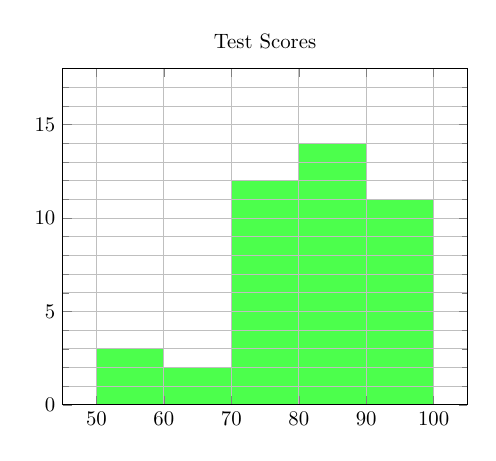
\begin{tikzpicture}[scale=0.75]
\begin{axis}[
    ymin=0, ymax=18,
    minor y tick num = 4,
    area style, grid=both, title=Test Scores
    ]
\addplot+[ybar interval,mark=no,fill=green!70] plot coordinates { (50, 3) (60, 2) (70, 12) (80, 14) (90, 11) (100, 9)};
\end{axis}
\end{tikzpicture}
\end{center}
\end{frame}

\begin{frame}{Example 1}
(d) What is the relative frequency of the 5th class?	\quad \onslide<3->{11/42}	
\begin{center}
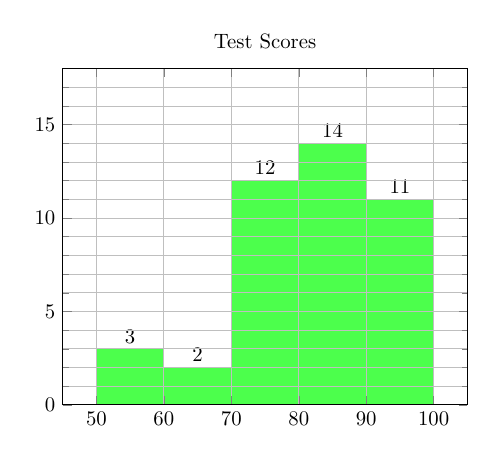
\begin{tikzpicture}[scale=0.75]
\begin{axis}[
    ymin=0, ymax=18,
    minor y tick num = 4,
    area style, grid=both, title=Test Scores
    ]
\addplot+[ybar interval,mark=no,fill=green!70] plot coordinates { (50, 3) (60, 2) (70, 12) (80, 14) (90, 11) (100, 9)};
\onslide<2->{
\node at (55,3.66) {3};
\node at (65,2.66) {2};
\node at (75,12.66) {12};
\node at (85,14.66) {14};
\node at (95,11.66) {11};
}
\end{axis}
\end{tikzpicture}
\end{center}
\end{frame}

\begin{frame}{Example 2}
Create a histogram from the measurements below. Use the minimum value as the lower class limit of the first class and use a class width of 2.	\newline\\
\begin{center}
\begin{tabular}{ccccc}
9& 2& 10& 1& 4	\\
5& 1& 6& 7& 4	\\
6& 5& 4& 8& 10	\\ 
3& 1& 2& 3& 9	\\
8& 6& 1& 1& 10
\end{tabular}
\end{center}
\onslide<2->{Use 1,3,5,7,9, and 11 as the lower class limits.}
\end{frame}

\begin{frame}{Example 2}
\begin{center}
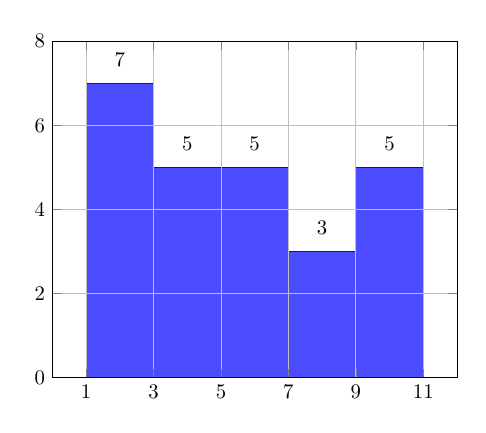
\begin{tikzpicture}[scale=0.75]
\begin{axis}[
    ymin=0, ymax=8,
    xtick = {1,3,...,11},
    % minor y tick num = 4,
    area style, grid=both, 
    ]
\addplot+[ybar interval,mark=no,fill=blue!70] plot coordinates { (1,7) (3,5) (5,5) (7,3) (9,5) (11,5)};
\onslide<2->{
\node at (2,7.55) {7};
\node at (4,5.55) {5};
\node at (6,5.55) {5};
\node at (8,3.55) {3};
\node at (10,5.55) {5};
}
\end{axis}
\end{tikzpicture}
\end{center}
\end{frame}

\begin{frame}{Example 3}
(a) \quad Given the histogram below of the weights of 200 dogs, find the total number of dogs whose weight is at least 34 pounds.	\newline\\
\begin{minipage}{0.7\textwidth}
\begin{tikzpicture}
\node at (0,0) {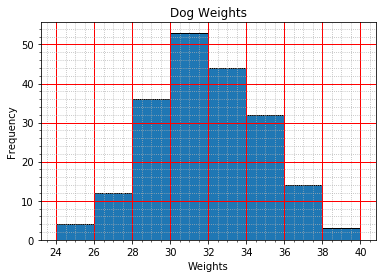
\includegraphics[scale=0.55]{../Images/dog_weights_hist.png}};
\onslide<2->{\node at (1.45,0.65) {32};}
\onslide<3->{\node at (2.15,-0.65) {14};}
\onslide<4->{\node at (2.9,-1.5) {3};}
\end{tikzpicture}
\end{minipage}
\hspace{0.25cm}
\begin{minipage}{0.2\textwidth}
\onslide<5->{Total: 49}
\end{minipage}
\end{frame}

\begin{frame}{Example 3}
(b) \quad What percentage of the dogs have weights between 26 and 28 pounds?	\newline\\
\begin{minipage}{0.7\textwidth}
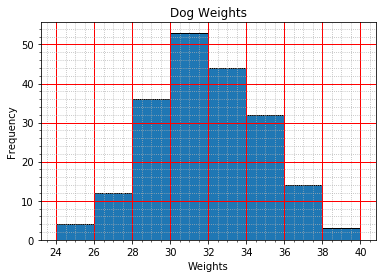
\includegraphics[scale=0.55]{../Images/dog_weights_hist.png}
\end{minipage}
\hspace{0.25cm}
\begin{minipage}{0.2\textwidth}
\onslide<2->{12/200} \\[10pt]
\onslide<3->{6\%}
\end{minipage}
\end{frame}


\begin{frame}{Some Common Histogram Shapes}
Uniform distribution:	\newline\\
\begin{center}
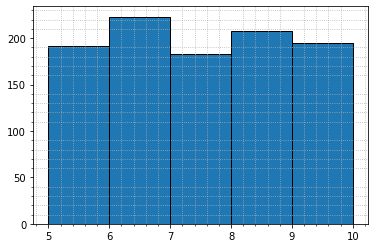
\includegraphics[scale=0.55]{../Images/uniform.png}
\end{center}
\end{frame}

\begin{frame}{Some Common Histogram Shapes}
Right (a.k.a. positively) skewed
\begin{center}
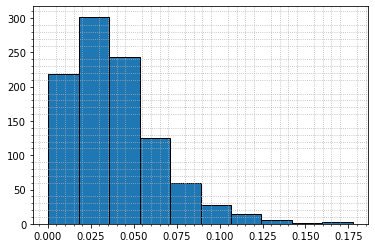
\includegraphics[scale=0.55]{../Images/positive_skewed.png}
\end{center}
\onslide<2->{\emph{Note}: Skewness refers to the \underline{tail}}
\end{frame}

\begin{frame}{Some Common Histogram Shapes}
Normal (a.k.a. bell-shaped)
\begin{center}
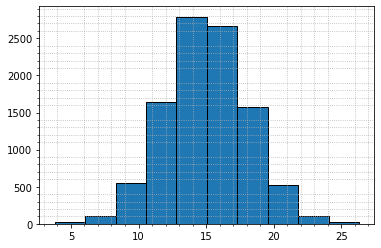
\includegraphics[scale=0.55]{../Images/normal1.png}
\end{center}
\end{frame}

\begin{frame}{Some Common Histogram Shapes}
Left (a.k.a. negatively) skewed
\begin{center}
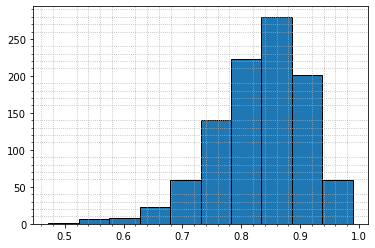
\includegraphics[scale=0.55]{../Images/negative_skewed.png}
\end{center}
\end{frame}

\begin{frame}{Cumulative Histogram Distributions}
The cumulative relative frequency histogram below shows a running total of relative frequencies of scores for a mathemathics test.
\begin{center}
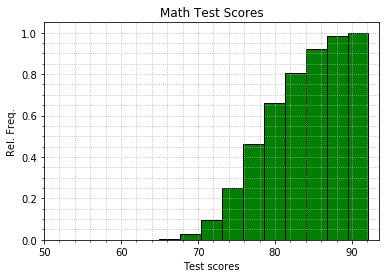
\includegraphics[scale=0.6]{../Images/cumulative_hist.png}
\end{center}
\end{frame}

\end{document}